% good graph for glucose and insulin effects after meals           http://en.wikipedia.org/wiki/File:Suckale08_fig3_glucose_insulin_day.png


% Aller voir les references du mail ayant pour objet "dissertation extract"


%wc latex: 
%begin  1606
%obj    
%end    
\section{Diabetes}

%%%%%%%%%%%%%%%%%%%%%%%%%%%%%%%%%%%%%%%%%%%%%%%%%%%%%%%%%%%%%%%%%%%%%%%%%%%%%%%%%%%%%%%%%%%%%%%%%%%%%%%%%%%%%%%%%%%%        CHAPTER 0   : A long term disorder                %%%%%%%%%%%%%%%%%%%%%%%%%%%%%%%%%%%%%%%%%%%%%%%%%%%%%%%%%%%%%%%%%%%%%%%%%%%%%%%%%%%%%%%%%%%%%%%%%%%%%%%%%%%%%%%%%%%%%%%%%%%%%%%%%%%%%%%%%%%%%%%%%%%%%%%%%%%%%%%%%%%%%%%%%%%%%%%%%%%%%%%%%%%%%%%%%%%%%%%%%%%%%%%%%%%%%%%%%%%%%%%%%%%%%%%%%%%%%%%%%%%%%%%%%%%%%%%%%%%%%%%%%%%%%%%%%%
\subsection{A long term disorder}%"Biological side"%}
We assume that "diabetes" stands for "type 1 diabetes" in the following section. Diabetes occurs when the body stops producing insulin, usually without any early-warning sign in the case of type 1 diabetes. The young patient is often admitted in the hospital with a very high level of sugar in blood, suffering from what is called hyperglycemia.
\paragraph{}

% #ref Type 1 diabetes, novo nordisk%
Nothing can be done to prevent the onset of diabetes, and research still doesn't know why the disease occur. Diabetes develops when the immune system starts destroying the cells of the pancreas involved in the creation of insulin. The immune system normally protects the body by destroying foreign substances such as bacteria. 

\subsubsection{Food and glucose regulation}
Glucose is an essential fuel for the organism, used by the organs such as muscles or the brain. Glucose comes from food and is released in the blood during digestion. Blood glucose regulation is done by two hormones: insulin and glucagon. No matter the individual had an important meal a couple of hours before or fasted all the day, blood glucose is always between 4 and 7 mmol/l. 
\\After a meal, blood glucose is high. Insulin is then released, making the blood level decrease till it reaches a normal level, while the extra glucose is stored in the liver and the organs. When the level of glucose becomes too low, glucagon is produced, and some glucose contained in the liver is release in the blood. 

\paragraph{Two insulins, two key functions}
%#ref nice graph p.20 of https://shop.diabetes.org.uk/usr/downloads/Carbs-Count-2012-reduced.pdf, can be used%
Insulin as an hypoglycemic hormone, which means that it makes blood glucose decrease. 
%Insulin is a hormone which is produced by the beta cells in the pancreas. Insulin acts like a key to unlock cells. It allows glucose in the blood stream to enter the cells. When insulin is not present, glucose cannot enter the cells and it builds up in the blood. %
Basal insulin and bolus insulin are the two types used for diabetes treatment. Bolus insulin is injected after each meal in order to compensate the amount of glucose absorbed by eating. It's a short acting insulin. However, a minimal amount of insulin is needed all day long because organs need a little insulin to be able to convert glucose into energy. For this purpose, basal insulin is injected once a day, it's a long acting insulin. 

%However, insulin plays another key role: making the glucose usable by the organs. %
\subsubsection{Symptoms}
High blood glucose is called hyperglycemia, and is due to a lack of insulin. Thus, muscles cannot turn blood glucose into energy to use it, given that insulin is needed for this process. Hyperglycemia is characterized by %(an extreme) 
tiredness due to a very high blood glucose. The body react trying to get rid of some glucose by the urines. Such a patient will need to drink large amounts of water and urinate unusually often. 

Low blood glucose is called hypoglycemia, and occurs in diabetics mainly because of too much insulin injected. The patient may feel dizzy, tired and can loose consciousness. Sugar, often in the form of carbohydrates, need to be eaten quickly in order to raise blood glucose to a normal level.  

\subsubsection{Treatment and diabetes management}
Daily insulin therapy is the only way to treat diabetes. Patients need to learn how to inject, and how much insulin they inject. "Carbohydrate counting" is a technique used to match insulin requirements with food intake. The principles of carbohydrate counting will be explained in section~\ref{sec:ccount}.
%%%%%%%%%%%%%%%%%%%%%%%%    ADDED
%\section{Management WARNING: added and to be changed}
%"Management. The basic elements of type 1 diabetes management are insulin administration (either by injection or insulin pump), nutrition management, physical activity, blood glucose testing, the avoidance of severe hypoglycemia, and the avoidance of prolonged hyperglycemia or DKA." %in http://ndep.nih.gov/media/youth_factsheet.pdf
%%%%%%%%%%%%%%%%%%%%%%%

\subsubsection{Long term effects and complications}
High and low blood glucose can be corrected with insulin therapy. Living with a poor blood glucose regulation has long term effects. Blood vessels are damaged, increasing the risk of heart diseases. Two other organs are often the first affected by long term high blood sugar, these are the eyes and feet. Sight loss and foot ulcers are more likely to occur if you have diabetes.  

\subsubsection{HbA1c}
HbA1c is used in diabetes management as an average blood glucose level. HbA1c stands for glycated haemoglobin, and is produced when glucose is fixed on haemoglobin molecules, which are the red blood cells in the blood stream. 
This value is different from blood glucose levels, which is a snapshot of the amount of glucose present in the blood at a given point in time. As red blood cells survive for 8 to 12 weeks, HbA1c is considered as an average measure of blood glucose. With the diabetes team, a patient tries to follow the target levels descibed in table~\ref{table:hba1cValues}.

\begin{table}
    \begin{tabular}{|l|l|l|}
    \hline
    Target Levels & HbA1c (\%) \\ \hline
    Non-diabetic          & 4 to 5.9\%                    \\ 
    People with diabetes       & 6.5\%                                         \\ 
    People with diabetes and greater hypoglycemia risk           & 7.5\% \\ \hline
    \end{tabular}
    
    \caption{Average values for HbA1c}
    \label{table:hba1cValues}
\end{table}


HbA1c is stable over 3 months, so it's usually tested each 3 months if the patient wants to improve his diabetes control, and every 6 months for routine examinations if diabetes control is good.

%%%%%%%%%%%%%%%%%%%%%%%%%%%%%%%%%%%%%%%%%%%%%%%%%%%%%%%%%%%%%%%%%%%%%%%%%%%%%%%%%%%%%%%%%%%%%%%%%%%%%%%%%%%%%%%%%%%        CHAPTER 0   : Psychological issues                %%%%%%%%%%%%%%%%%%%%%%%%%%%%%%%%%%%%%%%%%%%%%%%%%%%%%%%%%%%%%%%%%%%%%%%%%%%%%%%%%%%%%%%%%%%%%%%%%%%%%%%%%%%%%%%%%%%%%%%%%%%%%%%%%%%%%%%%%%%%%%%%%%%%%%%%%%%%%%%%%%%%%%%%%%%%%%%%%%%%%%%%%%%%%%%%%%%%%%%%%%%%%%%%%%%%%%%%%%%%%%%%%%%%%%%%%%%%%%%%%%%%%%%%%%%%%%%%%%%%%%%%%%%%%%%%%%
%\subsection{Enhancing diabetes management/"Psycological issues"}
\subsection{Psychological issues and diabetes management}

Adolescence represents a period of transition that brings about %OR (comes up with?) 
profound changes in a child's life, bringing physical, intellectual and psychological changes. Such changes are hard to deal with, and can be amplified by a conflicting relationship with parents. Being diagnosed with diabetes in such a period is especially challenging.
\\
For diabetics, adolescence with diabetes is complicated for several reasons. Physiological changes can induce insulin resistance, so patients with well managed diabetes can suddenly change to poorly controlled diabetes. Lack of well-being and psychological issues can seriously affect diabetes management. 
\\
\paragraph{Medical effects}
The hormons that causes growth during adolescence are also known to induce an insulin-resistance~\cite{HelpChildTeenTD1}.

%http://jdrf.org/life-with-t1d/type-1-diabetes-information/control-and-management/helping-your-child-or-teen-live-with-type-1-diabetes/

Growth Hormone, involved in the growth of bone and muscle mass during puberty, is accounted to be responsible for this resistance. As a result, glucose levels tend to be higher, and insulin doses usually need to be increased to suit the patient's needs. 
This results in highs and lows. Adrealine worsens the situation as sudden falls in blood glucose trigger adrenaline emission, which results in the release of stored glucose. 
Experiencing such high variations in blood glucose often result in a strong feeling of lost of control.

\\
Due to adolescence, nutritional requirements also change while the body experience the greatest amount of growth in height and weight. Daily food intake have to increase to meet the new body's needs, and teenagers often struggle with a hungry feeling between meals.  

%\paragraph{Management || treatment changes || treatment efficiency (adherence?)}
\paragraph{Adolescence and changes in diabetes management}
Due to this insulin resistance and the profound changes of adolescence, treatment need to be readapted, usually with higher insulin doses. Hypoglycemia can result, and a frustrating feeling of constant hunger. \\A good example of treatment adaption is the way practicians are recommanded to advise adolescents about snacking. \\
%REFERENCE Bon livre ! Pour des conseils, etc : http://books.google.fr/books?id=GVjW7m9cE1QC&pg=PA20&lpg=PA20&dq=adolescence+hunger+snack+diabetes&source=bl&ots=gGlnWXTytD&sig=VevM2h2Oy8Xe8a8uNMUO4P-0gR8&hl=fr&sa=X&ei=aJD3UbiGAseV7AbR94FY&ved=0CDoQ6AEwAQ#v=onepage&q=adolescence%20hunger%20snack%20diabetes&f=false
In order to reduce cravings between meals, practicians can advise teenagers about snacking. We can cite the use of free food, which is food with negligible amount of carbohydrates, ie 20 or less calories per serving. This kind of food can be reasonably consumed as often as wanted by the diabetic patient \cite{tu1993assessment}. However, the more adolescents are growing, the more energy they need, which makes free-food-based snacks inadequate. Thus, patients are advised to have a good-sized snack with an insulin injection in order to prevent lows and keep glucose levels under control, instead of simply tacking only one small snack, and being hungry quickly after, or tacking multiple spaced snacks without insulin injections, resulting in hyperglyecmia risks. A good snacking policy is related with higher quality diabetes management, with lower HbA1c levels~\cite{delahanty1993role}, especially for snacks in the evening or consistent night snacks.
\\
On top of that, children and adolescents misconceptions about snacking need to be cleared to lead to good snacking habits. Usually, they all know that non-free-food snacks beyond the meal plan are not allowed by their caregivers. Considering it a \`bad\' behaviour, they tend not to mention extra-snacks when discussing their insulin plan with the diabetes team. Snacking is a good example of a kind of treatment change due to adolescence.

%=EFFICIENCY=
%* Motivational therapy : gives long term neutral (not positive) results on HbA1c at 36 months(Article "ismail2009motivational")Motivational enhancement therapy with and without cognitive behaviour therapy to treat type 1 diabetes: the long-term outcomes of a randomised controlled trial)
%=> A study performed on patients in 8 diabetes centres in the UK showed that a motivational behavioral therapy associated with a cognitive behavioural therapy resulted in an improvement of patient glycaemic control, with 50\% reduction of the HbA1c levels 12 months after the beginning of the study, compared to patients that were only provided with usual care. However, 24 months after the beginning of the study, there were no significant difference between the groups in HbA1c levels.
%The improvement due to the motivational and cognitive behavioural therapy disappeared after 24 months, so only short term effects of the therapy can be highlighted.
\\

\paragraph{Psychological issues: depression and diabetes}
%=Gender=
\\
%=Depression=
\\
%*Effects of depression : depression and bad food habits (Article "ahola2009depression") Depression and sense of coherence are associated with food intake and compliance with dietary guidance in type 1 diabetes
\\
Adolescence with diabetes is psychologically burdensome. 
\\
Research showed that the prevalence of depressed individuals is higher in a diabetic population (24\%) than in a non-diabetic population (17\%) in a 3,010 individuals study~\cite{goldney2004diabetes}. Moreover, suffering from diabetes and depression (all) together have important consequences on quality of life : if depression has a higher effect than diabetes on quality of life, the effect of diabetes with depression is higher than the combination of both. 
\\
While depression can be treated with good results by antidepressants~\cite{Goodnick2000}, negative effects were reported on glycemic control when they were used by diabetics ~\cite{Lustman2002917}. Complications due to the combination of diabetes and depression lead to very important costs : total health care for diabetics suffering from depression were 4.5 higher than those for diabetics without depression ~\cite{egede2002comorbid}.
\\
Furthermore, figures of depression associated with diabetes in youth are alarming~\cite{Grey2002907}:\\
``Children with diabetes have a two-fold greater prevalence of depression, and adolescents up to three-fold greater, than youth without diabetes.''\\
Linked with a poorer metabolic control and serious long-term complications, depression may alter adherence to the diabetic care and induce an insulin-resistance because of an hypersecretion of cortisol. Family and support seems to play a key role in depression associated with diabetes, so behavioral therapies, including family approaches, could prevent or treat efficiently depression for such patients.
\\
Finally, well being promotion and psychological follow-ups seem crucial in order to prevent this kind of complications when dealing with diabetic youngsters.
\\


%=Self image=

%\paragraph{Social issues}

%Concerning psychological issues, associations between a better mental health, a better control of glucose values and a more positive approach to diabetes management are highlighted in~\cite{hackworth2013predictors}. A relashionship between risky behaviour and poor diabetes control was also found. 

%=Family support=
\\
%=Peer relashionships=
\\

%\subsubsection{Social and psychological issues}
\subsubsection{The lack of support and education about diabetes}
Family Support represents a key point of the success of diabetes management. A study~\cite{maas2013interrelationships} revealed that depression in teenagers is associated with poor blood glucose control and parenting stress. The relationship found in ~\cite{clayton2013impact}  goes beyond that, revealing that mother's depression affects more diabetes management than a teenager's own depressed feelings.
\\Thus, parents' education appears as a crucial point affecting diabetes management. However, 
this article~\cite{familyFactors} showed that the importance of peer support, especially for the mother is extremely important. Indeed, there was a close link between adolescents with good glucose control and the parent's feeling of being supported by their peers, especially among mothers. This can be explained by the fact that mothers that make the largest effort in diabetes management consider that the burden of diabetes is too high, and that they have this feeling of being not supported enough by peers. The study highlighted the fact that peers, which might be relatives or the parent's friends, are not educated enough about diabetes to be able to take care of the child. Therefore, all the responsability and efforts remains in the parent's hands. This situation is partly due to a lack of accessible solutions to educate such friends and relatives about diabetes. The software we aim to produce in this project may provide a solution for the general public.\\
            

%\subsubsection{Diabetes at School}




%%%%%%%%%%%%%%%%%%%%%%%%%%%%%%%%%%%%%%%%%%%%%%%%%%%%%%%%%%%%%%%%%%%%%%%%%%%%%%%%%%%%%%%%%%%%%%%%%%%%%%%%%%%%%%%%%%%%        CHAPTER 0   : Patient education                %%%%%%%%%%%%%%%%%%%%%%%%%%%%%%%%%%%%%%%%%%%%%%%%%%%%%%%%%%%%%%%%%%%%%%%%%%%%%%%%%%%%%%%%%%%%%%%%%%%%%%%%%%%%%%%%%%%%%%%%%%%%%%%%%%%%%%%%%%%%%%%%%%%%%%%%%%%%%%%%%%%%%%%%%%%%%%%%%%%%%%%%%%%%%%%%%%%%%%%%%%%%%%%%%%%%%%%%%%%%%%%%%%%%%%%%%%%%%%%%%%%%%%%%%%%%%%%%%%%%%%%%%%%%%%%%%%
\subsection{Patient education}

[NEW] Results in a study concerning their knowledge about diabetes : example of bad level of knowledge about carb count:
\\"A second skill activity provided a list of foods along with their portion size and asked participants to use the carbohydrate counting method to create an appropriate breakfast, lunch, and dinner, each containing four carbohydrate servings. Participants completed this task correctly 50\% for breakfast, 39\% for lunch, and 44\% for dinner on their first attempt. The percent correct increased to 60\% with repeated attempts for all three meals (data not shown)."~\cite{herrejon2009creation}

%This Msc project is led by the University of Manchester and the Royal Manchester Children’s Hospital. 

When a child is first diagnosed, it is admitted to the hospital for a few days, usually 3 to 6 days. Medical care is provided at the very beginning and during the stay according to the condition. At the same time, the diabetes team, including doctors, nurses and dieticians are meeting him regularly. 

\\
The nurse teaches the patient mainly about general knowledge concerning the disease, and all the practical knowledge to be able to practice self care diabetes management. A dietician focuses mainly on carbohydrate counting, and helps the child to figure out an appropriate diet, with advices on nutrition and sport.
%%%%%%%%%%%%%%%%%%%%%%%%%%%%%       WARNING IFFALSE
\iffalse


\section{Hba1c, complications, ketones ?}
The paper
~\cite{HBA1Ckilpatrick2012rise}
%%%%%%%%%%%%%%%%%%%%%%%%%%%%%%%

\subsubsection{In the literature}
\subsubsection{Education on the ward}
In order to get a better understanding of patient's experience and expectations, I went to the hospital to attend the educational sessions. I was taught as if I was a real patient, and invited to ask the questions a teenager could ask. Trying to react as a 'normal' patient was a way to collect the amount of knowledge they have, and the approach that is used to teach them.
\\In Royal Manchester Children’s Hospital, there is 4 sessions, 2 with the diabetes nurse, and 2 with the dietician. It may be underestimating to say that patients are often upset while they attend these sessions because they learnt only one or two days before that they were suffering from diabetes, a long term disorder.

%%%%%%%%%%%%%%%%%%%%%%%%%%%%%%%%%%%%%%%%%%%%%%%%%%%%%%%%%%%%%%%%%%%%


\begin{figure}[h]
  \caption{A page from the Carbs and Cals book}
  \centering
  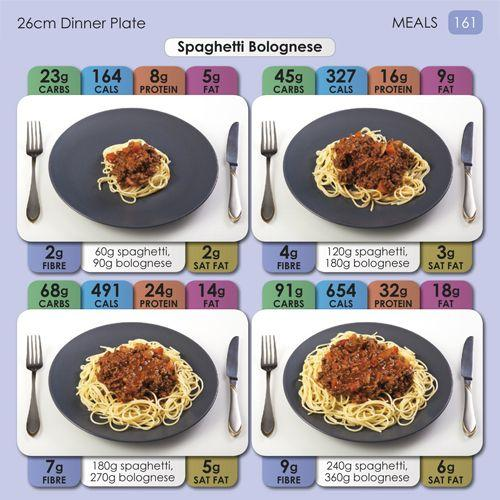
\includegraphics[scale=0.9]{bookImage}
  \label{fig:bookImage}
\end{figure}



%%%%%%%%%%%%%%%%%%%%%%%%%%%%%       WARNING IFFALSE
\fi

%%%%%%%%%%%%%%%%%%%%%%%%%%%%%%%%%%
%%%     Carbohydrate counting
%%%%%%%%%%%%%%%%%%%%%%%%%%%%%%%%%%
\subsection{Carbohydrate counting} 
\label{sec:ccount}
This technique is used to manage blood glucose. \paragraph{Carbohydrate} is a nutrient, contained in some food and drink. During digestion, carbohydrate breaks down into glucose, which is then used as energy by the body. 
We can classify carbohydrates in two main types: starchy carbohydrates and sugars. 
"Starchy carbohydrates" come from sources such as pasta, bread, rice and potatoes. "Sugars" designate sucrose, fructose (found in fruits) and lactose (found in dairy foods). Patients need to take bolus insulin to cover the glucose derived from carbohydrates during meals~\cite{carbcountPdf}. 
\paragraph{}To find how much bolus insulin they need to take, diabetics should know:
\begin{enumerate}
\item How much insulin is needed for a certain amount of carbohydrates. This ratio is individual to each person, and tends to increase during adolescence.
\item The amount of carbohydrates they will eat and drink for this meal.
\end{enumerate}

\begin{figure}[h]
  \centering
  \caption{Example of a meal with corresponding carbohydrate levels~\cite{refhowtocarbPic}}
  \includegraphics[scale=1.2]{mealcount}
  \label{fig:mealcount}
\end{figure}

%Nice example in page 30 of the book%
For instance, if a patient has:
\begin{itemize}
\item A ratio of 1:10, which means that 1 unit of insulin is needed to cover 10 grams of carbohydrates in food
\item The food as shown in figure~\ref{fig:mealcount} as a meal
\end{itemize}



He will then sum the carbohydrates of the meal as follows:

$\begin{array}{l l l}
    Carbs & \quad  = 0 + 15 + 15 + 4 + 12   & \quad \textrm{Carbs in eggs, raspberry, bread, peanut butter and milk}\\
         & \quad = 46 g   
  \end{array}$
  
\paragraph{}
The ratio of 1:10 gives the units of insulin needed with a simple division of the total amount of carbohydrates by the ratio, rounded to the nearest whole number, as follows:

$\begin{array}{l l l}
    InsulinUnits & \quad  = 46/10 \\
         & \quad = 4.6  \\
         & \quad 5 units & \quad \textrm{rounded value}
  \end{array}$
\paragraph{}
In this example, 5 units of bolus insulin need to be injected. 

\paragraph{Correction doses of insulin} are added to the injection if blood glucose is high compared to the target values in table \ref{table:targetValues}. This may occur if the patient didn't take enough insulin before the previous meal or had some snack between two meals. Most people will need 1 unit of bolus insulin to reduce blood glucose levels by 2–3 mmol/l ~\cite{carbcountPdf}. 


\begin{table}
    \begin{tabular}{|l|l|l|}
    \hline
    Target Levels by Type & Before meals (pre prandial) & 2 hours after meals (post prandial) \\ \hline
    Non-diabetic          & 4.0 to 5.9 mmol/L           & under 7.8 mmol/L                    \\ 
    Type 1 diabetes       & 4 to 7 mmol/L               & under 9 mmol/L                      \\ \hline
    \end{tabular}
    
    \caption{International Diabetes Federation's target ranges for people without diabetes}
    \label{table:targetValues}
\end{table}


\paragraph{}In the previous example, if blood glucose before the meal was 10 mmol/L, and the patient's target value is 6 mmol/L. If one unit of insulin lowers the blood glucose levels by 2 mmol/L, the target is to lower the blood glucose by 4 mmol/L. Thus, 2 units of insulin will reach the target level.
\\This corrective dose of insulin needs to be added to the insulin counted by the carbohydrate couting method, so the toal amount of injected insulin is 5 + 2 = 7 units of insulin.

\paragraph{How to know the amount of carb in a meal ?}
There are various ways to figure out the amount of carbohydrates available in a given food:
\begin{itemize}
\item The patient can read food labels, where the amount of carbohydrates for 100g or for a given portion is indicated.
\item Reference lists can be used. These lists are available in some leaflets provided by the hospital, and in the very comprehensive reference book~\cite{cheyette2010carbs} given to each newly diagnosed patient. 
%screen book https://shop.diabetes.org.uk/usr/catalogue/pi_442.jpg
\end{itemize}

In the children's hospital, this book is widely used because portion sizes in a standard size plate are shown in pictures, which makes it really easy to find the correct amount by visual comparizon as can be seen in figure~\ref{fig:bookImage}. A mobile application using this principle is also available for iPhone, Android and BlackBerry. Using easy-to-learn and visual methods fits the needs of diabetes management for children patients.
\begin{figure}[h]
  \centering
  \caption{Visual comparizon}
  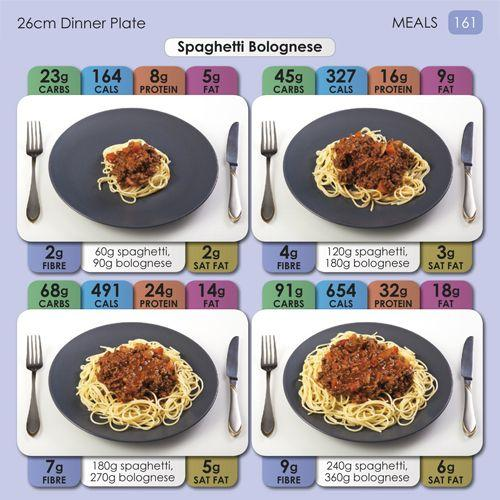
\includegraphics[scale=1.2]{bookImage.jpg}
  \label{fig:bookImage}
\end{figure}

\subsection{Motivations}

Intensive diabetes treatment has positive consequences on the onset and evolution of complications, postponing them~\cite{dcct1994effect}. Rethinopathy occurence was reduced by 53\% for patients followed on average for 7.3 years. On the other hand, patients that followed normal therapy without specific glycemic targets and patients following an intensive therapy that aimed for a near-normal glycemic level with 3 or more insulin injections a day were fewer than 1\% to have an amputation or become blind because of diabetes. [explain somewhere more in detail, with the figures, and keep only the summary here]

"Moreover, suboptimal glycemic control that is established during early adolescence[3] may be very difficult to change, even with state-of-the-art behavioral intervention.[4]"

